In Figs.~\ref{fig:distNLO1}--\ref{fig:distNLO3}, several differential distributions are shown.
All these predictions are performed at NLO accuracy at the order $\mathcal{O}(\alphas\alpha^6)$.
In the upper panel, the absolute predictions are shown while in the lower panel, the ratio with respect to the full predictions are displayed.
The band corresponds to a seven-points variation of the factorisation and renormalisation scales.

We start with Fig.~\ref{fig:distNLO1} which displays the invariant mass (left) and the rapidity separation (right) of the two tagging jets.
For high invariant mass, all predictions agree rather well.
On the other hand, for low invariant mass, the hierarchy present at the level of the cross section is here reproduced.
The VBS-approximated predictions ({\sc Bonsay} and {\sc Powheg-Box}) are lower than the full calculation ({\sc MoCaNLO}+{\sc Recola}).
The full calculation is rather well approximated by the hybrid VBS approximation implemented in {\sc MG5\_aMC}.
Finally, {\sc VBFNLO} which includes also $s$-channel contributions provides larger predictions at low invariant mass.
For the rapidity difference between the two tagging jets, the hierarchy between the predictions is rather similar.
Therefore, depending on the approximation used, it can vary by $\pm7\%$ and $\pm4\%$ with respect to the full computation at low invariant mass and low rapidity difference for the tagging jets, respectively

 \begin{figure*}[hbt!]
   \centering
   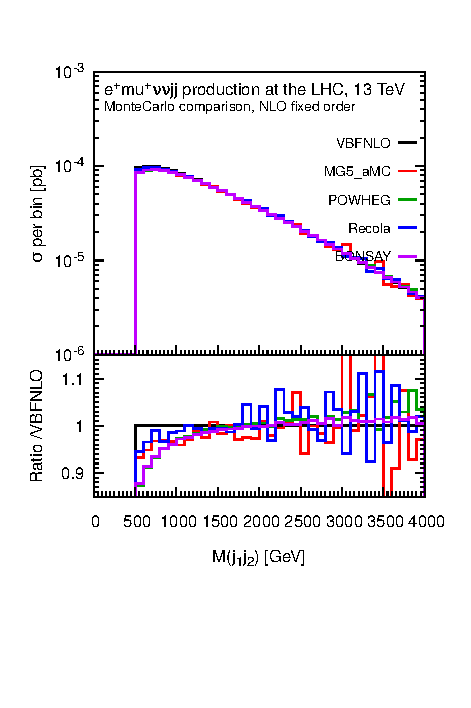
\includegraphics[width=0.4\textwidth,angle=0,clip=true,trim={0.4cm 2cm 0.cm 1.cm}]{figures/NLO/mjj_NLO.pdf}
   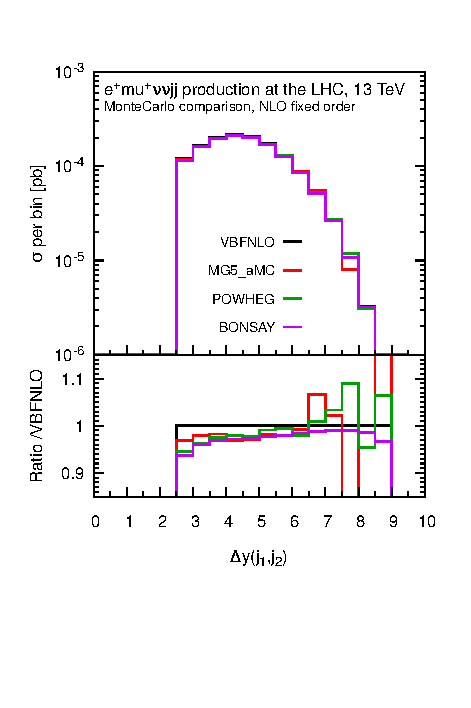
\includegraphics[width=0.4\textwidth,angle=0,clip=true,trim={0.4cm 2cm 0.cm 1.cm}]{figures/NLO/dyj1j2_NLO.pdf}
\caption{\label{fig:distNLO1} Differential distributions in the invariant mass (left) and rapidity difference of the two tagging jets (right).
The LHC process considered is ${\rm p}{\rm p}\to\mu^+\nu_\mu{\rm e}^+\nu_{\rm e}{\rm j}{\rm j}$ at NLO accuracy at $\mathcal{O}(\alpha_{\rm s}\alpha^6)$.
The description of the different programs used can be found in Sec.~\ref{subsec:codedescr}.
The upper plots provide the absolute value for each prediction while the lower plots present all predictions normalised to {\sc MoCaNLO}+{\sc Recola} which is the full predictions.
The band corresponds to a seven-points scale variation of the renormalisation and factorisation scale.
The predictions are obtained in the fiducial region described in Sec.~\ref{subsec:inputpar}.
}
\end{figure*}

Concerning the transverse momentum (left) and rapidity (right) of the hardest jet shown in Fig.~\ref{fig:distNLO2}, the situation is rather different.
While {\sc MG5\_aMC} is very close to the full prediction for low transverse momentum, it departs from it 
at larger transverse momentum by about $10\%$.
This is in contrast with the VBS-approximated predictions such as {\sc Bonsay}, {\sc Powheg}, and {\sc VBFNLO} which are lower than the full computation at low transverse momentum and higher for larger transverse momentum.
The difference at high transverse momentum between the latter predictions and the full computation can be attributed to EW Sudakov logarithms that become large in this phase-space region.
While, the predictions of {\sc Bonsay} and {\sc Powheg} are rather close over the whole range, the one of {\sc VBFNLO} is very drifferent at low transverse momentum where it is even higher than the full computation.
We note that for the transverse momentum of the second hardest jet, the predictions from {\sc MG5\_aMC} are in good agreement with the other VBS-approximated predictions.
% Finally, {\sc VBFNLO} predicts higher rates over the whole range apart from around $200\GeV$ where it is in perfect agreement with the complete calculation.
Concerning the rapidity of the hardest jet, {\sc VBFNLO} is in good agreement with {\sc MoCaNLO}+{\sc Recola} in the rapidity range $|y_{j_1}| < 3$.
For larger rapidity, the other codes constitute a better description of the full process at order $\mathcal{O}(\alpha_{\rm s}\alpha^6)$.

 \begin{figure*}[hbt!]
   \centering
   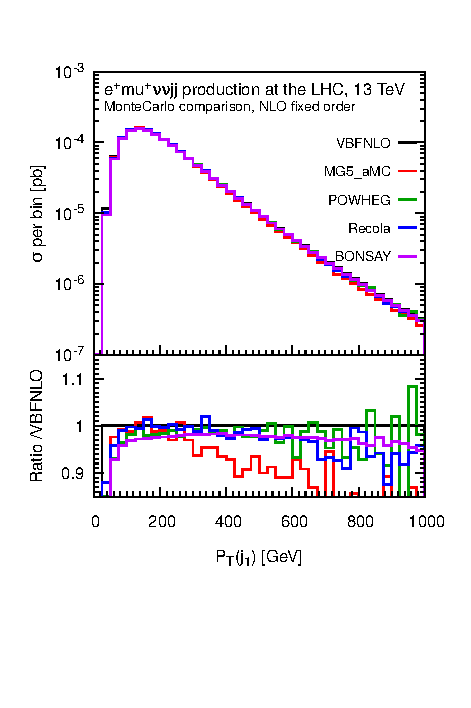
\includegraphics[width=0.4\textwidth,angle=0,clip=true,trim={0.4cm 2cm 0.cm 1.cm}]{figures/NLO/ptj1_NLO.pdf}
   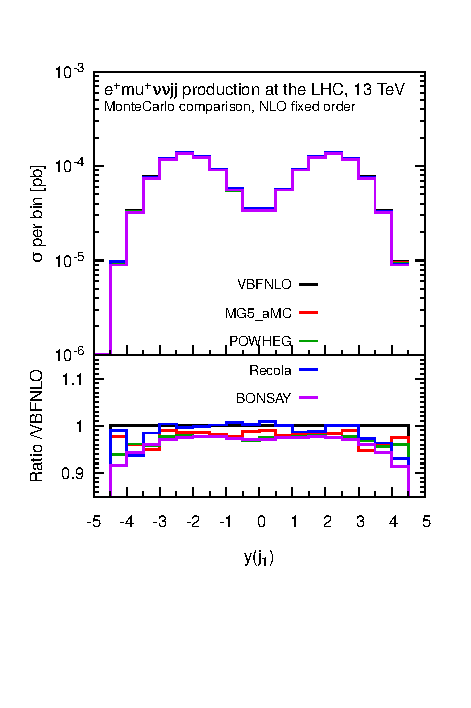
\includegraphics[width=0.4\textwidth,angle=0,clip=true,trim={0.4cm 2cm 0.cm 1.cm}]{figures/NLO/yj1_NLO.pdf}
\caption{\label{fig:distNLO2} Differential distributions in the transverse momentum (left) and rapidity of the hardest jet (right).
The LHC process considered is ${\rm p}{\rm p}\to\mu^+\nu_\mu{\rm e}^+\nu_{\rm e}{\rm j}{\rm j}$ at NLO accuracy at $\mathcal{O}(\alpha_{\rm s}\alpha^6)$.
The description of the different programs used can be found in Sec.~\ref{subsec:codedescr}.
The upper plots provide the absolute value for each prediction while the lower plots present all predictions normalised to {\sc MoCaNLO}+{\sc Recola} which is the full predictions.
The band corresponds to a seven-points scale variation of the renormalisation and factorisation scale.
The predictions are obtained in the fiducial region described in Sec.~\ref{subsec:inputpar}.
}
\end{figure*}

The last set of differential distributions is the invariant mass of the two charged lepton (left) and the Zeppenfeld variable for the anti-muon (right).
Concerning the comparison of the predictions, both distributions display a rather similar behaviour.
Indeed, the hierarchy mentioned previously is here respected and enhanced towards high invariant mass or high Zeppenfeld variable.
The predictions of {\sc MoCaNLO}+{\sc Recola} and {\sc VBFNLO} are in rather good agreement for both distributions for the kinematic range displayed here.
The other three VBS approximations are close to each other within few per cents.

 \begin{figure*}[hbt!]
   \centering
   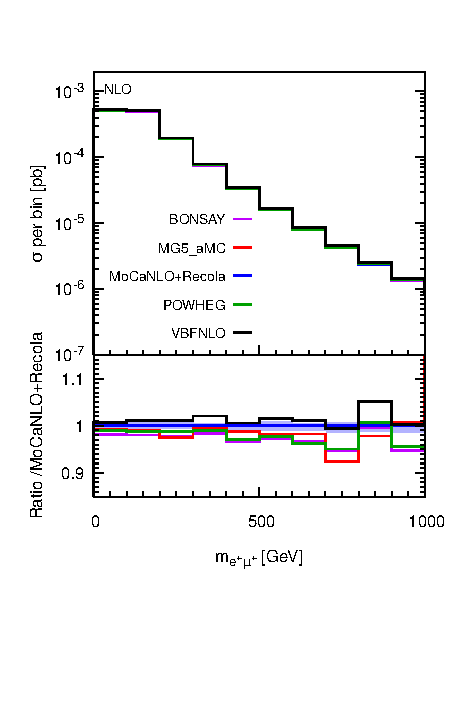
\includegraphics[width=0.4\textwidth,angle=0,clip=true,trim={0.4cm 2cm 0.cm 1.cm}]{figures/NLO/mll_NLO.pdf}
   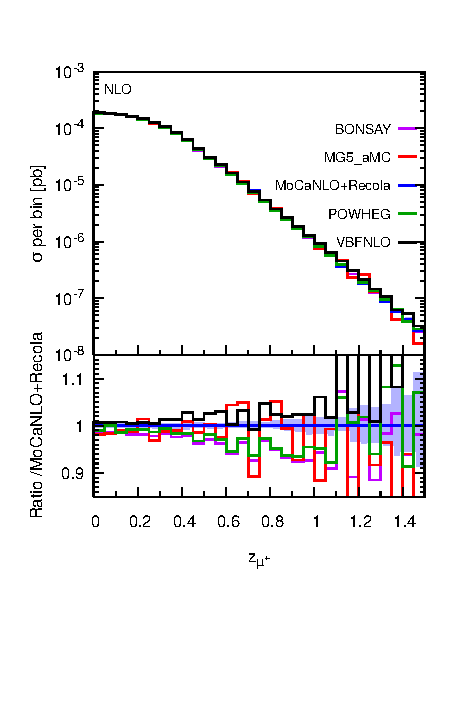
\includegraphics[width=0.4\textwidth,angle=0,clip=true,trim={0.4cm 2cm 0.cm 1.cm}]{figures/NLO/zmu_NLO.pdf}
\caption{\label{fig:distNLO3} Differential distributions in the invariant mass of the two charged leptons (left) and Zeppenfeld variable for the muon (right).
The LHC process considered is ${\rm p}{\rm p}\to\mu^+\nu_\mu{\rm e}^+\nu_{\rm e}{\rm j}{\rm j}$ at NLO accuracy at $\mathcal{O}(\alpha_{\rm s}\alpha^6)$.
The description of the different programs used can be found in Sec.~\ref{subsec:codedescr}.
The upper plots provide the absolute value for each prediction while the lower plots present all predictions normalised to {\sc MoCaNLO}+{\sc Recola} which is the full predictions.
The band corresponds to a seven-points scale variation of the renormalisation and factorisation scale.
The predictions are obtained in the fiducial region described in Sec.~\ref{subsec:inputpar}.
}
\end{figure*}

In the end, the quality of the VBS approximations is good up to $10\%$ in the fiducial region.
These differences are larger than those at LO.

The contributions from the $s$-channel amplitude can be sizeable especially at low invariant mass for the two tagging jets (comparing the predictions of {\sc VBFNLO} against the ones of {\sc Bonsay} and {\sc Powheg}).
This can be explained by the fact that $s$-channel contributions are less suppressed at NLO.
In the real, an extra gluon-jet can be radiated from any of the charged particles while the two quarks originating from the W-boson decay can be recombined in a single jet.
Therefore, the jet requirements ($ m_{\Pj \Pj} >  500\GeV$ and $|\Delta y_{\Pj \Pj}| > 2.5$) that were suppressing $s$-channel contributions at LO are partially lifted with the inclusion of a third jet at NLO.
Such an effect has also been observed for top--antitop production in the lepton+jet channel at NLO QCD \cite{Denner:2017kzu}.

% As the $s$-channel contributions are sizeable, their interferences with the $t$/$u$-channel can be of similar size in the phase-space region where the former are large.
In phase-space regions where the $s$-channel contributions are sizeable their interference with the $t/u$-channel can be of similar size.
This can be observed by comparing the predictions of {\sc VBFNLO} against the ones of {\sc MG5\_aMC}.

Finally, the effect of EW corrections and NF contributions in the virtual corrections are usually small.
But they can be relatively large (about $10\%$) for large transverse momentum of the hardest jet.
These high-energy region of the phase space are where EW Sudakov logarithms become large.
Nonetheless these regions are rather suppressed and thus these effects are hardly visible at the level of the cross section.
